\documentclass[12pt]{report} % You can use 'article' or 'book' class as well

\usepackage{graphicx} % For including images
\usepackage{amsmath}
\usepackage{amssymb}
\usepackage{caption}
\usepackage{forest}
\usepackage{hyperref}
\usepackage{multicol}
\usepackage{pgfplots}
\usepackage{tikz}
\usepgfplotslibrary{fillbetween}
\pgfplotsset{compat=1.18}

\begin{document}

% Title page
\begin{titlepage}
	\centering
	\vspace*{1cm} % Adjusts vertical space for the image
	% Insert your image (use the actual path and filename of your image)
	\includegraphics[width=0.3\textwidth]{../images/KMITL Logo.png} % Adjust width as needed

	\vspace{1cm} % Vertical space after the image
	{\LARGE \textbf{Week 12 Homework}} \\[0.5cm] % Title
	\vspace{0.5cm}
	{\large \textbf{Probability Model and Data Analysis}} \\[0.5cm]
    {\large \textbf{Software Engineering Program,}} \\[0.5cm]
	{\large \textbf{Department of Computer Engineering,}} \\[0.5cm]
	{\large \textbf{School of Engineering, KMITL}} \\[1cm]
    {\Large 67011352 Theepakorn Phayonrat} \\[0.5cm] % Authors (Use \\ the separate authors)
\end{titlepage}

\section*{Homework of Pairs of Random Variables-Joint PMF}

\subsection*{Question 1}

\noindent (4.2.1) Random variables $X$ and $Y$ have the joint PMF

\[
    P_{X,Y}(x, y) =
    \begin{cases}
        cxy & x = 1, 2, 4; \indent  y = 1, 3 \\
        0 & otherwise \\
    \end{cases}
\]

\noindent (a) What is the value of the constant $c$? \\
\noindent (b) What is $P[Y < X]$? \\
\noindent (c) What is $P[Y > X]$? \\
\noindent (d) What is $P[Y = X]$? \\
\noindent (e) What is $P[Y = 3]$? \\

\subsection*{Solution}


\noindent (a)

\begin{center}
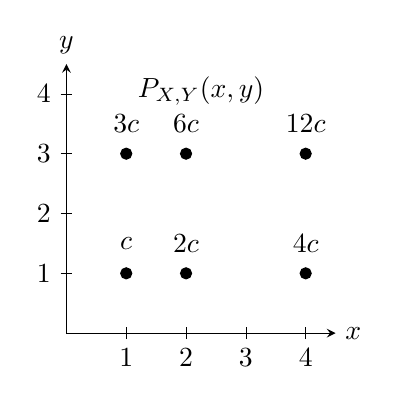
\begin{tikzpicture}
\begin{axis}[
    xmin=0, xmax=4.5,
    ymin=0, ymax=4.5,
    xtick={0,1,2,3,4},
    ytick={0,1,2,3,4},
    axis lines=left,
    xlabel={$x$},
    ylabel={$y$},
    width=5cm,
    height=5cm,
    tick style={black},
    axis lines=middle,
    enlargelimits=false,
    axis on top,
    xlabel style={at={(axis description cs:1,0)}, anchor=west}, % put X at rightmost
    ylabel style={at={(axis description cs:0,1)}, anchor=south} % put Y at topmost
]

\addplot[only marks, mark=*, mark size=2pt] coordinates {
    (1, 1)
    (1, 3)
    (2, 1)
    (2, 3)
    (4, 1)
    (4, 3)
};

% Labels
\node at (axis cs:1,1.5) {$c$};
\node at (axis cs:2,1.5) {$2c$};
\node at (axis cs:4,1.5) {$4c$};

\node at (axis cs:1,3.5) {$3c$};
\node at (axis cs:2,3.5) {$6c$};
\node at (axis cs:4,3.5) {$12c$};

% Title above
\node at (rel axis cs:0.5,0.90) {$P_{X,Y}(x,y)$};

\end{axis}
\end{tikzpicture}
\end{center}

\begin{align*}
    \therefore \sum_{x = 1, 2, 4} \sum_{y = 1, 3} P_{X, Y}(x, y) & = c \sum_{x = 1, 2, 4} X \sum_{y = 1, 3}Y \\
    1 & = c (1(1 + 3) + 2(1 + 3) + 4(1 + 3)) = 28c \\
    \therefore c & = \frac{1}{28} \\
\end{align*}

\newpage

\noindent From earlier, $c = \frac{1}{28}$. \\

\[
    P_{X,Y}(x, y) =
    \begin{cases}
        \frac{1}{28} xy & x = 1, 2, 4; \indent  y = 1, 3 \\
        0 & otherwise \\
    \end{cases}
\]

\noindent (b) \\

\begin{align*}
    P[Y < X] & = P_{X, Y}(2, 1) + P_{X, Y}(3, 1) + P_{X, Y}(4, 3) \\
    & = \frac{1}{28}(2)(1) + \frac{1}{28}(3)(1) + \frac{1}{28}(4)(3) \\
    & = \frac{2}{28} + \frac{4}{28} + \frac{12}{28} \\
    \therefore P[Y < X] & = \frac{18}{28} = \frac{9}{14} \\
\end{align*}


\noindent (c) \\

\begin{align*}
    P[Y > X] & = P_{X, Y}(3, 1) + P_{X, Y}(3, 2) \\
    & = \frac{1}{28}(3)(1) + \frac{1}{28}(3)(2) \\
    \therefore P[Y > X] & = \frac{3}{28} + \frac{6}{28} = \frac{9}{28} \\
\end{align*}

\noindent (d) \\

\begin{align*}
    P[Y = X] & = P_{X, Y}(1, 1) \\
    & = \frac{1}{28}(1)(1) \\
    \therefore P[Y = X] & = \frac{1}{28} \\
\end{align*}

\newpage

\noindent (e) \\

\begin{align*}
    P[Y = 3] & = P_{X, Y}(1, 3) + P_{X, Y}(2, 3) + P_{X, Y}(4, 3) \\
    & = \frac{1}{28}(1)(3) + \frac{1}{28}(2)(3) + \frac{1}{28}(4)(3) \\
    & = \frac{3}{28} + \frac{6}{28} + \frac{12}{28} \\
    \therefore P[Y = 3] & = \frac{21}{28} = \frac{3}{4} \\
\end{align*}

\newpage

\subsection*{Question 2}

\noindent For two of fair coin, let $X$ equal the total number of tails
and let $Y$ equal the number of heads on the last flip. Find the joint
PMF $P_{X,Y}(x, y)$ \\

\subsection*{Solution}

\[
\begin{forest}
for tree={
  grow'=right,                 % Tree grows left to right
  draw, circle,                % All nodes are circles with border
  minimum size=1.25em,          % Consistent node size
  inner sep=1pt,               % Padding inside nodes
  parent anchor=east,          % Connect parent from right side
  child anchor=west,           % Connect child from left side
  edge path={
    \noexpand\path [draw, \forestoption{edge}]
    (!u.parent anchor) -- (.child anchor)\forestoption{edge label};
  },
  s sep=15mm,                  % Sibling separation
  l sep=20mm                   % Level separation
}
% Tree starts here
[, fill=gray!30,
    [$H$, edge label={node[midway,above] {0.50}}
        [H, edge label={node[midway,above] {0.50}}
            [$\alpha$]
        ]
        [T, edge label={node[midway,below] {0.50}}
            [$\beta$]
        ]
    ]
    [$T$, edge label={node[midway,below] {0.50}}
        [H, edge label={node[midway,above] {0.50}}
            [$\gamma$]
        ]
        [T, edge label={node[midway,below] {0.50}}
            [$\delta$]
        ]
    ]
]
\end{forest}
\]

\begin{align*}
    \alpha \rightarrow X = 0, Y = 1, P_{X, Y}(0, 1) = 0.25 \\
    \beta \rightarrow X = 1, Y = 0, P_{X, Y}(1, 0) = 0.25 \\
    \gamma \rightarrow X = 1, Y = 1, P_{X, Y}(1, 1) = 0.25 \\
    \delta \rightarrow X = 2, Y = 1, P_{X, Y}(2, 1) = 0.25 \\
\end{align*}

\[
\begin{array}{c|c c}
    P_{X, Y}(x, y) & y = 0 & y = 1 \\ \hline
    x = 0 & 0   & \tfrac{1}{4} \\
    x = 1 & \frac{1}{4} & \frac{1}{4} \\
    x = 2 & \frac{1}{4} & 0 \\
\end{array}
\\ \indent
P_{X,Y}(x,y) =
\begin{cases}
    \frac{1}{4} & x = 0 \indent  y = 1\\
    \frac{1}{4} & x = 1 \indent y = 0\\
    \frac{1}{4} & x = 1 \indent y = 1\\
    \frac{1}{4} & x = 2 \indent y = 1\\
0 & otherwise
\end{cases}
\]


\newpage

\section*{Homework of Marginal PMF}

\subsection*{Question 1}

\noindent Given the random variables $X$ and $Y$ in Problem 4.2.1, find \\

\noindent (a) The marginal PMFs $P_{X}(x)$ and $P_{Y}(y)$ \\
\noindent (b) The expected values $E[X]$ and $E[Y]$ \\
\noindent (c) The standard deviation $\sigma_{X}$ and $\sigma_{Y}$ \\

\subsection*{Solution}

\noindent (a)

\begin{align*}
    P_{X}(x) & = \sum_{y} P_{X, Y}(x, y) \\
    & = P_{X, Y}(x, 1) + P_{X, Y}(x, 3) \\
    & = \frac{1}{28}(x)(1) + \frac{1}{28}(x)(3) \\
    \therefore P_{X}(x) & = \frac{4x}{28} = \frac{x}{7} \\
\end{align*}
$$\therefore P_{X}(1) = \frac{1}{7} \indent \therefore P_{X}(2) = \frac{2}{7} \indent \therefore P_{X}(4) = \frac{4}{7} \\$$

\begin{align*}
    P_{Y}(y) & = \sum_{y} P_{X, Y}(x, y) \\
    & = P_{X, Y}(1, y) + P_{X, Y}(2, y) + P_{X, Y}(4, y) \\
    & = \frac{1}{28}(1)(y) + \frac{1}{28}(2)(y) + \frac{1}{28}(4)(y) \\
    \therefore P_{Y}(y) & = \frac{7y}{28} = \frac{y}{4} \\
\end{align*}
$$\therefore P_{Y}(1) = \frac{1}{4} \indent \therefore P_{Y}(3) = \frac{3}{4} \\$$

\newpage

\noindent (b)

\begin{align*}
    E[X] & = \sum_{x} x P_{X}(x) \\
    & = 1(\frac{1}{7}) + 2(\frac{2}{7}) + 4(\frac{4}{7}) \\
    & = \frac{1 + 4 + 16}{7} \\
    \therefore E[X] & = \frac{21}{7} = 3 \\
\end{align*}

\begin{align*}
    E[Y] & = \sum_{y} y P_{Y}(y) \\
    & = 1(\frac{1}{4}) + 3(\frac{3}{4}) \\
    & = \frac{1 + 9}{4} \\
    \therefore E[Y] & = \frac{10}{4} = \frac{5}{2} = 2.5 \\
\end{align*}

\noindent (c) \\

\noindent To find $\sigma_{X}$ and $\sigma_{Y}$, we need to find
$Var[X]$ and $Var[Y]$

\begin{align*}
    E[X^{2}] & = \sum_{x} x^{2} P_{X}(x) \\
             & = 1^{2}(\frac{1}{7}) + 2^{2}(\frac{2}{7}) + 4^{2}(\frac{4}{7}) \\
    & = \frac{1 + 8 + 64}{7} \\
    \therefore E[X^{2}] & = \frac{73}{7} \\
\end{align*}

\newpage

\begin{align*}
    Var[X] & = E[X^{2}] - (E[X])^{2} \\
    & = \frac{73}{7} - 3^{2} \\
    & = \frac{73}{7} - \frac{63}{7} \\
    \therefore Var[X] & = \frac{10}{7} \\
    \therefore \sigma_{X} & = \sqrt{\frac{10}{7}} \\
\end{align*}

\begin{align*}
    E[Y^{2}] & = \sum_{y} y^{2} P_{Y}(y) \\
             & = 1^{2}(\frac{1}{4}) + 3^{2}(\frac{3}{4}) \\
    & = \frac{1 + 27}{4} \\
    \therefore E[Y^{2}] & = \frac{28}{4} = 7 \\
\end{align*}

\begin{align*}
    Var[Y] & = E[Y^{2}] - (E[Y])^{2} \\
    & = 7 - 2.5^{2} \\
    & = 7 - 6.25 \\
    \therefore Var[Y] & = 0.75 = \frac{3}{4} \\
    \therefore \sigma_{Y} & = \sqrt{\frac{3}{4}} = \frac{\sqrt{3}}{2} \\
\end{align*}

\newpage

\subsection*{Question 2}

\noindent (4.2.2) Random variables $X$ and $Y$ have hoint PMF

\[
    P_{X,Y}(x, y) =
    \begin{cases}
        c|x + y| & x = -2, 0, 2; \indent  y = -1, 0, 1 \\
        0 & otherwise \\
    \end{cases}
\]

\noindent (a) What is the value of the constant $c$? \\
\noindent (b) What is $P[Y < X]$? \\
\noindent (c) What is $P[Y > X]$? \\
\noindent (d) What is $P[Y = X]$? \\
\noindent (e) What is $P[X < 1]$? \\

\subsection*{Solution}

\noindent (a)

\begin{center}
\begin{tikzpicture}
\begin{axis}[
    xmin=-2.5, xmax=2.5,
    ymin=-2.5, ymax=2.5,
    xtick={-2,-1,0,1,2},
    ytick={-2,-1,0,1,2},
    axis lines=left,
    xlabel={$x$},
    ylabel={$y$},
    width=10cm,
    height=10cm,
    tick style={black},
    axis lines=middle,
    enlargelimits=false,
    axis on top,
    xlabel style={at={(axis description cs:1,0.5)}, anchor=west}, % put X at rightmost
    ylabel style={at={(axis description cs:0.5,1)}, anchor=south} % put Y at topmost
]

\addplot[only marks, mark=*, mark size=2pt] coordinates {
    (-2, -1)
    (-2, 0)
    (-2, 1)
    (0, -1)
    (0, 0)
    (0, 1)
    (2, -1)
    (2, 0)
    (2, 1)
};

% Labels
\node at (axis cs:-1.75,-0.75) {$3c$};
\node at (axis cs:-1.75,0.25) {$2c$};
\node at (axis cs:-1.75,1.25) {$c$};

\node at (axis cs:0.25,-0.75) {$c$};
\node at (axis cs:0.25,0.25) {$0$};
\node at (axis cs:0.25,1.25) {$c$};

\node at (axis cs:2.25,-0.75) {$c$};
\node at (axis cs:2.25,0.25) {$2c$};
\node at (axis cs:2.25,1.25) {$3c$};

% Title above
\node at (rel axis cs:0.75,0.90) {$P_{X,Y}(x,y)$};

\end{axis}
\end{tikzpicture}
\end{center}

\newpage

$$\therefore \sum_{x = -2, 0, 2} \sum_{y = -1, 0, 1} P_{X, Y}(x, y) & = c \sum_{x = 1, 2, 4} \sum_{y = 1, 3}|X + Y|$$ \\
\[
    \begin{array}{c|c c c}
        |X + Y| & Y = -1 & Y = 0 & Y = 1 \\ \hline
        X = -2 & |-2 + (-1)| = 3 & |-2 + 0| = 2 & |-2 + 1| = 1 \\
        X = 0 & |0 + (-1)| = 1 | & |0 + 0| = 0 & |0 + 1| = 1 \\
        X = 2 & |2 + (-1)| = 1 | & |2 + 0| = 2 & |2 + 1| = 1 \\
    \end{array}
\]


\begin{align*}
\therefore \sum_{x = -2, 0, 2} \sum_{y = -1, 0, 1} P_{X, Y}(x, y) & = c(3 + 2 + 1 + 1 + 0 + 1 + 1 + 2 + 3) \\
1 & = c(14) \\
\therefore c & = \frac{1}{14} \\
\end{align*}

\noindent From earlier, $c = \frac{1}{14}$. \\

\[
    P_{X,Y}(x, y) =
    \begin{cases}
        \frac{1}{14} |x + y| & x = -2, 0, 2; \indent  y = -1, 0, 1 \\
        0 & otherwise \\
    \end{cases}
\]

\newpage

\noindent (b)

\begin{align*}
P[Y < X] & = P_{X, Y}(0, -1) + P_{X, Y}(2, -1) + P_{X, Y}(2, 0) + P_{X, Y}(2, 1) \\
    & = \frac{1}{14}|0 + (-1)| + \frac{1}{14}|2 + (-1)| + \frac{1}{14}|2 + 0| + \frac{1}{14}|2 + 1| \\
    & = \frac{1}{14} + \frac{1}{14} + \frac{2}{14} + \frac{3}{14} \\
    \therefore P[Y < X] & = \frac{7}{14} = \frac{1}{2} \\
\end{align*}

\noindent (c)

\begin{align*}
    P[Y > X] & = P_{X, Y}(-2, -1) + P_{X, Y}(-2, 0) + P_{X, Y}(-2, 1) + P_{X, Y}(0, 1) \\
    & = \frac{1}{14}|-2 + (-1)| + \frac{1}{14}|-2 + 0| + \frac{1}{14}|-2 + 1| + \frac{1}{14}|0 + 1| \\
    & = \frac{3}{14} + \frac{2}{14} + \frac{1}{14} + \frac{1}{14} \\
    \therefore P[Y > X] & = \frac{7}{14} = \frac{1}{2} \\
\end{align*}

\noindent (d)

\begin{align*}
    P[Y = X] & = P_{X, Y}(-2, -1) \\
    & = \frac{1}{14}|0 + 0| \\
    & = \frac{0}{14} \\
    \therefore P[Y = X] & = 0 \\
\end{align*}

\newpage

\noindent (e)

\begin{align*}
    P[X < 1] & = P[X = 0] + P[X = -1] \\
    & = \frac{1}{14}|0 + -1| + \frac{1}{14}|0 + 0| + \frac{1}{14}|0 + 1| + P[Y = -1] \\
    & = \frac{1}{14} + 0 + \frac{1}{14} + P[Y = -1] \\
    & = \frac{2}{14} + P[Y = -1] \\
    & = \frac{2}{14} + \frac{1}{14}|-1 + (-2)| + \frac{1}{14}|-1 + 0| + \frac{1}{14}|-1 + 2| \\
    & = \frac{2}{14} + \frac{3}{14} + \frac{1}{14} + \frac{1}{14} \\
    \therefore P[X < 1] & = \frac{7}{14} = \frac{1}{2} \\
\end{align*}

\subsection*{Question 3}

\noindent Given the random variables $X$ and $Y$ in Problem 4.2.2, find \\

\noindent (a) The marginal PMFs $P_{X}(x)$ and $P_{Y}(y)$ \\
\noindent (b) The expected values $E[X]$ and $E[Y]$ \\
\noindent (c) The standard deviation $\sigma_{X}$ and $\sigma_{Y}$ \\

\newpage

\subsection*{Solution}

\noindent (a)

\begin{align*}
    P_{X}(x) & = \sum_{y} P_{X, Y}(x, y) \\
    & = P_{X, Y}(x, -1) + P_{X, Y}(x, 0) + P_{X, Y}(x, 1) \\
    & = \frac{1}{14}|x + (-1)| + \frac{1}{14}|x + 0| + \frac{1}{14}|x + 1| \\
    \therefore P_{X}(x) & = \frac{|x - 1| + |x| + |x + 1|}{14} \\
\end{align*}

\begin{align*}
    P_{X}(-2) & = \frac{|-2 - 1| + |-2| + |-2 + 1|}{14} \\
    & = \frac{|-3| + |-2| + |-1|}{14} \\
    \therefore P_{X}(-2) & = \frac{3 + 2 + 1}{14} = \frac{6}{14} = \frac{3}{7} \\
\end{align*}

\begin{align*}
    P_{X}(0) & = \frac{|0 - 1| + |0| + |0 + 1|}{14} \\
    & = \frac{|-1| + |0| + |1|}{14} \\
    \therefore P_{X}(0) & = \frac{1 + 0 + 1}{14} = \frac{2}{14} = \frac{1}{7} \\
\end{align*}

\begin{align*}
    P_{X}(2) & = \frac{|2 - 1| + |2| + |2 + 1|}{14} \\
    & = \frac{|1| + |2| + |3|}{14} \\
    \therefore P_{X}(2) & = \frac{1 + 2 + 3}{14} = \frac{6}{14} = \frac{3}{7} \\
\end{align*}

\newpage

\begin{align*}
    P_{Y}(y) & = \sum_{y} P_{X, Y}(x, y) \\
    & = P_{X, Y}(-2, y) + P_{X, Y}(0, y) + P_{X, Y}(2, y) \\
    & = \frac{1}{14}|-2 + y| + \frac{1}{14}|0 + y| + \frac{1}{14}|2 + y| \\
    \therefore P_{Y}(y) & = \frac{|-2 + y| + |y| + |2 + y|}{14}|-2 + y| \\
\end{align*}

\begin{align*}
    P_{Y}(-1) & = \frac{|-2 - (-1)| + |-1| + |-2 + -1|}{14} \\
    & = \frac{|-1| + |-1| + |-3|}{14} \\
    \therefore P_{Y}(-1) & = \frac{1 + 1 + 3}{14} = \frac{5}{14} = \frac{2.5}{7} \\
\end{align*}

\begin{align*}
    P_{Y}(0) & = \frac{|-2 - 0| + |0| + |-2 + 0|}{14} \\
    & = \frac{|-2| + |0| + |-2|}{14} \\
    \therefore P_{Y}(0) & = \frac{2 + 0 + 2}{14} = \frac{4}{14} = \frac{2}{7} \\
\end{align*}

\begin{align*}
    P_{Y}(1) & = \frac{|-2 - 1| + |1| + |-2 + 1|}{14} \\
    & = \frac{|-3| + |1| + |-1|}{14} \\
    \therefore P_{Y}(1) & = \frac{3 + 1 + 1}{14} = \frac{5}{14} = \frac{2.5}{7} \\
\end{align*}

\newpage

\noindent (b)

\begin{align*}
    E[X] & = \sum_{x} x P_{X}(x) \\
    & = -2(\frac{3}{7}) + 0(\frac{1}{7}) + 2(\frac{3}{7}) \\
    & = \frac{-6 + 0 + 6}{7} \\
    \therefore E[X] & = 0 \\
\end{align*}

\begin{align*}
    E[Y] & = \sum_{y} y P_{Y}(y) \\
    & = -1(\frac{2.5}{7}) + 0(\frac{2}{7}) + 1(\frac{2.5}{7}) \\
    & = \frac{-2.5 + 0 + 2.5}{7} \\
    \therefore E[Y] & = 0 \\
\end{align*}

\noindent (c) \\

\noindent To find $\sigma_{X}$ and $\sigma_{Y}$, we need to find
$Var[X]$ and $Var[Y]$

\begin{align*}
    E[X^{2}] & = \sum_{x} x^{2} P_{X}(x) \\
    & = (-1)^{2}(\frac{3}{7}) + 0^{2}(\frac{1}{7}) + 1^{2}(\frac{3}{7}) \\
    & = \frac{3 + 0 + 3}{7} \\
    \therefore E[X^{2}] & = \frac{6}{7} \\
\end{align*}

\newpage

\begin{align*}
    Var[X] & = E[X^{2}] - (E[X])^{2} \\
    & = \frac{6}{7} - 0^{2} \\
    & = \frac{6}{7} - 0 \\
    \therefore Var[X] & = \frac{6}{7} \\
    \therefore \sigma_{X} & = \sqrt{\frac{6}{7}} \\
\end{align*}

\begin{align*}
    E[Y^{2}] & = \sum_{y} y^{2} P_{Y}(y) \\
    & = (-2)^{2}(\frac{2.5}{7}) + 0^{2}(\frac{2}{7}) + 2^{2}(\frac{2.5}{7}) \\
    & = \frac{5 + 0 + 5}{7} \\
    \therefore E[Y^{2}] & = \frac{10}{7} \\
\end{align*}

\begin{align*}
    Var[Y] & = E[Y^{2}] - (E[Y])^{2} \\
    & = \frac{10}{7} - 0^{2} \\
    & = \frac{10}{7} - 0 \\
    \therefore Var[Y] & = \frac{10}{7} \\
    \therefore \sigma_{Y} & = \sqrt{\frac{10}{7}} \\
\end{align*}

\end{document}
